\documentclass{beamer}
\usepackage{amsmath}
\usepackage{amssymb}
\usepackage{pgf}
\usepackage{tikz}
\usepackage{listings}
\usepackage{color}
\usepackage{nicefrac}
\usetikzlibrary{matrix}
\usetheme{boxes}
\newcommand{\fig}{./figures} % common figure path
\newcommand{\dbbslsh}{\textbackslash \textbackslash} % common figure path
\newenvironment{myblock}[3]{%
\definecolor{smtbx}{rgb}{0.64,0.76,0.68}
\setbeamercolor{block body}{#2}
\setbeamercolor{block title}{#3}
\begin{block}{#1}}{\end{block}}
\newcommand{\frnzplt}{FranzPlot }
\DeclareMathSymbol{\shortminus}{\mathbin}{AMSa}{"39}

\title[Curve e Sup. - Lab 3]{Curve e Superfici per il Design \\ Laboratorio - 4}
\author[Prof. Parolini]{Prof. Nicola Parolini}
%\institute[dimat]{Long Inst.}
\date{7 Novembre 2019}

\begin{document}

\begin{frame}
\maketitle
\end{frame}

\begin{frame}
\frametitle{Materiali}
Il materiale per l'esercitazione di oggi:
\begin{itemize}
\item Questa presentazione \\ (\texttt{Materiale Didattico/Laboratori/lab 4/lab4\_testo.pdf});
%\item Il file \texttt{es\_dado\_ref.toml} con l'esercizio risolto della passata esercitazione.
\item L'eseguibile del \frnzplt \\ (\texttt{Software/Franzplot 19.08 - Windows.exe})
\end{itemize}
\end{frame}


\section{Riepilogo}

\begin{frame}
\frametitle{Riepilogo}
    Per scrivere una retta in forma parametrica necessito di un \textbf{vettore direttore}
    e di un \textbf{punto appartente alla retta} (a volte chiamato \textit{termine noto}).

    \vspace{0.2cm}
    Sia $\mathbf v$ il vettore direttore e sia $\mathbf P$ il punto appartenente alla retta,
    allora la forma parametrica sar\`a $r(t) = \mathbf v t + \mathbf P$, con $t\in \mathbb{R}$.
    
    Scritto come sistema lineare:
\begin{displaymath}
    r(t) :\begin{cases} x = v_x t + P_x\\ y = v_y t + P_y \\z = v_z t + P_z \end{cases}
\quad t\in \mathbb{R}
\end{displaymath}

    \vspace{0.2cm}
    Il nome del parametro \`e arbitrario (tipicamente useremo $t$ o $s$).
    
    \`E sempre importante specificare l'intervallo di appartenenza.
\end{frame}

\begin{frame}
    \frametitle{Rette in \frnzplt}
    Per disegnare una qualsiasi curva parametrica in \frnzplt introduciamo i nodi \texttt{Geometries > Curve} e \texttt{Parameters > Interval}.

    \vspace{0.25cm}
    Il nodo \texttt{Interval} ci permette di definire il nome del parametro e l'intervallo cui appartiene.

    \vspace{0.25cm}
    Nel nodo \texttt{Curve} andiamo a inserire le coordinate $x$, $y$ e $z$ in funzione del parametro usato nel nodo \texttt{Interval}. Prendiamo ad esempio
    la seguente curva:

$$
r: \quad \left\{
\begin{array}{lcr}
x&=&3t+1\\
y&=&t-3\\
z&=&-2t
\end{array}
\right.
    \quad t\in \left[ \shortminus 10, 10 \right]
$$
    \end{frame}
    
\begin{frame}
    \frametitle{Rette in \frnzplt}
    Per visualizzare questa curva, creeremo il seguente grafo:
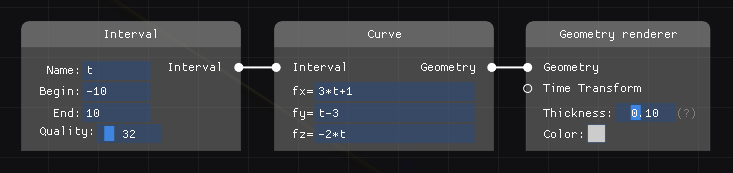
\includegraphics[width = 0.9\textwidth]{\fig/lab4_intro.png}
    L'output del nodo \texttt{Curve} \`e una Geometria, e come tale possiamo applicargli trasformazioni o animazioni.

    Una curva \`e una una Geometria 1D, possiamo usare lo slider \texttt{thickness} per modificare lo spessore usato nella visualizzazione.

    \vspace{0.5cm}
    Nota: nel nodo \texttt{Interval} non \`e possibile selezionare l'intero $\mathbb R$, quindi per \textbf{visualizzare} le rette scegliamo sempre un intervallo
    con valori sufficientemente grandi.

    \end{frame}

\section{Esercizi}
\begin{frame}
    \frametitle{Esercizio 1}

Date le seguenti rette nello spazio si calcoli, se esiste, il punto di intersezione:

$$
r:\left\{
\begin{array}{l}
x=3t+1\\
y=t-3\\
z= -2t
\end{array}
\right ., \qquad w:\left\{
\begin{array}{l}
x=s+3\\
y=4\\
z=-s+5
\end{array}
\right .
$$

    con $t, s \in \mathbb R$

    (Suggerimento: voglio che $r_x = w_x, \quad r_y = w_y, \quad r_z = w_z$)
    
    \vspace{1cm}
    Le rette sono perpendicolari?

    \end{frame}
    
\begin{frame}
    \frametitle{Esercizio 1 - i}

    Quando voglio trovare l'intersezione tra due curve \textit{qualsiasi}, devo imporre che
    i valori delle coordinate $x$, $y$ e $z$ siano uguali.
$$\left\{\begin{array}{l}
          3t+1=s+3\\
          t-3=4\\
          -2t=-s+5
         \end{array}\right.
$$

    Risolvo il sistema lineare: \\
        $\Rightarrow$ \textbf{Se} trovo una soluzione, allora le rette si intersecano in un punto.
$$
    \left\{\begin{array}{l}
          3t+1=s+3\\
          t=7\\
          s=2t+5
         \end{array}\right . 
$$
\end{frame}

\begin{frame}
    \frametitle{Esercizio 1 - ii}
    Ho ricavato il valore di $t$, lo sostituisco nella terza riga per trovare $s$
$$
    \left\{\begin{array}{l}
          3t+1=s+3\\
          t=7\\
          s=2\cdot7+5 = 19
         \end{array}\right . 
$$
    E per finire sostituisco $t$ e $s$ nella prima riga: \textbf{devo} essere sicuro che anche la prima equazione sia soddisfatta
$$
    \left\{\begin{array}{l}
          3\cdot7 + 1 = 19 + 3 \\
          t=7\\
          s=19
         \end{array}\right . 
    \quad
    \left\{\begin{array}{l}
          22=22\\
          t= 7\\
          s= 19
         \end{array}\right . 
$$

Posso confermare che le rette si intersecano.
Sostituisco $t=7$ nella retta $r$ per ottenere l'intersezione: $P=(22,4,-14)$.

\end{frame}

\begin{frame}
\frametitle{Esercizio 1 - iii}

Se guardiamo i vettori direttori, abbiamo:
$$
\mathbf{v} = \left[
\begin{array}{c}
3\\
1\\
-2
\end{array}
\right]
\qquad
    \mathbf{u} = \left[
\begin{array}{c}
1\\
0\\
-1
\end{array}
\right]
$$

Controlliamo se le direzioni formano un angolo retto:
$$
    \mathbf{v} \cdot \mathbf{u}
    =
    \left[
\begin{array}{c}
3\\
1\\
-2
\end{array}
\right]
\cdot
\left[
\begin{array}{c}
1\\
0\\
-1
\end{array}
\right]
= 3 + 0 + 2 = 5
$$
Quindi le rette non sono perpendicolari.
\end{frame}

\begin{frame}
\frametitle{Esercizio 2}

Siano assegnate le rette $r$ e $s$ di equazione
$$
r: \quad \left\{
\begin{array}{lcr}
x&=&3t-3\\
y&=&t-2\\
    z&=&-2t+4
\end{array}
\right. \qquad \qquad s: \quad \left\{
\begin{array}{lcr}
x&=&t\\
y&=&t-1\\
z&=&2t-2
\end{array}
\right.
$$

    \begin{itemize}
    \item $r$ ed $s$ sono perpendicolari? 
    \item Si visualizzino le rette $r$ e $s$ usando \frnzplt
    \end{itemize}
    
    \vspace{0.75cm}
    (Reminder: due rette sono perpendicolari se sono incidenti e le loro direzioni formano un angolo retto)
\end{frame}

\begin{frame}
\frametitle{Esercizio 2 - i}

Se guardiamo i vettori direttori, abbiamo:
$$
\mathbf{v} = \left[
\begin{array}{c}
3\\
1\\
-2
\end{array}
\right]
\qquad
    \mathbf{u} = \left[
\begin{array}{c}
1\\
1\\
2
\end{array}
\right]
$$

Controlliamo se le direzioni formano un angolo retto:
$$
\mathbf{v}  \cdot  \mathbf{u}
    = \left[
\begin{array}{c}
3\\
1\\
-2
\end{array}
\right]
\cdot
 \left[
\begin{array}{c}
1\\
1\\
2
\end{array}
\right]
= 3 + 1 - 4 = 0
$$
Le direzioni formano un angolo retto.
In 2D questo sarebbe sufficiente a garantire che le rette siano perpendicolari,
mentre in 3D \textbf{dobbiamo sempre controllare che le rette abbiano un punto in comune}.

\end{frame}

\begin{frame}
\frametitle{Esercizio 2 - ii}
Nota: \`e necessario cambiare ``nome'' del parametro della seconda retta!
$$
\left\{
\begin{array}{rcl}
    3t-3 &=& s\\
    t-2 &=& s-1\\
    -2t+4&=&2s -2
\end{array}
\right.
$$

Metto in evidenza $s$ dalla prima equazione e la sostituisco nella seconda e terza riga
$$
\left\{
\begin{array}{l}
    s = 3t-3\\
    t-2 = s-1\\
    -2t+4=2s -2
\end{array}
\right.
\quad
\left\{
\begin{array}{l}
    s = 3t-3\\
    t-2 = 3t - 3 -1\\
    -2t+4=6t - 6 -2
\end{array}
\right.
$$
\end{frame}

\begin{frame}
\frametitle{Esercizio 2 - iii}
Svolgo le somme e sposto i termini in $t$ a sinistra:
$$
\left\{
\begin{array}{l}
    s=3t-3\\
    2t=2\\
    8t=12
\end{array}
\right.
\quad
\left\{
\begin{array}{l}
    s=3t-3\\
    t=1\\
    t=\nicefrac{3}{2}
\end{array}
\right.
$$

    \vspace{0.75cm}
La seconda e terza riga evidenziano che il sistema lineare non ha soluzione, quindi
le due rette non si intersecano! \\
    $\Rightarrow$ Le due rette non sono perpendicolari, sono sghembe.
\end{frame}

\begin{frame}
\frametitle{Esercizio 2 - iv}

    \vspace{-1cm}
\begin{center}
\begin{tikzpicture}
\node(img1){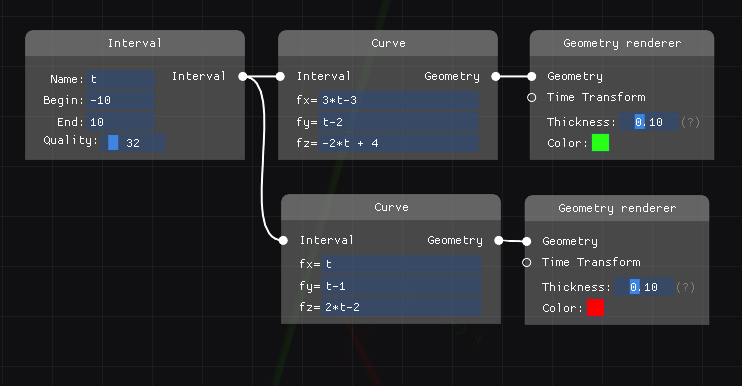
\includegraphics[width=0.8\textwidth]{\fig/lab4_es1_graph.png}};
\node(img2) at (img1.south west){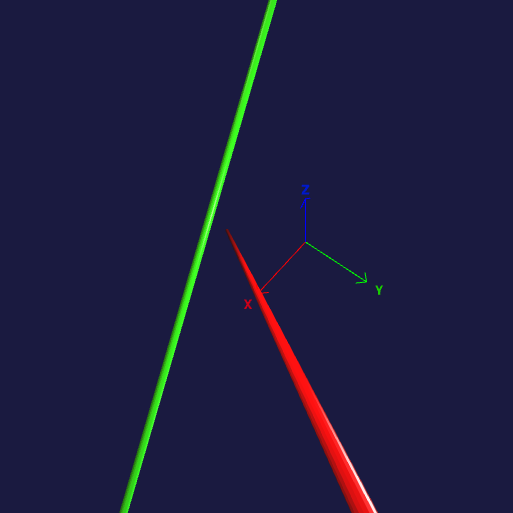
\includegraphics[width=0.4\textwidth]{\fig/lab4_es1_scene.png}};
\end{tikzpicture}
\end{center}

\end{frame}

\begin{frame}
\frametitle{Esercizio 3}
Dati i punti
$$
\mathbf{P}=\left[
\begin{array}{c}
0\\
-2\\
-1
\end{array}
\right]
\qquad
\mathbf{R}=\left[
\begin{array}{c}
3\\
-1\\
2
\end{array}
\right] \qquad
\mathbf{S}=\left[
\begin{array}{c}
-2\\
1\\
0
\end{array}
\right] 
$$
si calcolino:
    \begin{itemize}
    \item una rappresentazione parametrica della retta $r$ \\ passante per $\mathbf{P}$ e $\mathbf{R}$.
    \item una rappresentazione parametrica della retta $s$ \\ passante per $\mathbf{P}$ e $\mathbf{S}$.
    \end{itemize}
    
Le due rette sono perpendicolari?
\end{frame}

\begin{frame}
\frametitle{Esercizio 3 - i}

La rappresentazione di $r$ e $s$ non sono uniche; la pi\`u immediata per $r$ sar\`a:
\begin{itemize}
        \item vettore direttore $\overrightarrow{PR}$
        \item retta passante per $P$
\end{itemize}
Dai dati ricaviamo che:
$$
\overrightarrow{PR} = \left[
\begin{array}{c}
3\\
1\\
3
\end{array}
\right]
\qquad
\mathbf P = \left[
\begin{array}{c}
0\\
-2\\
-1
\end{array}
\right]
$$
quindi 
$$r: \quad \left\{
\begin{array}{rcl}
x&=&3t+0\\
y&=&1t-2\\
z&=&3t-1
\end{array}
\right. \quad t\in \mathbb{R}
$$
\end{frame}

\begin{frame}
\frametitle{Esercizio 3 - ii}

Alla stessa maniera, per $s$ scegliamo:
\begin{itemize}
        \item vettore direttore $\overrightarrow{PS}$
        \item retta passante per $P$
\end{itemize}
Dai dati ricaviamo che:
$$
\overrightarrow{PS} = \left[
\begin{array}{c}
-2\\
3\\
1
\end{array}
\right]
\qquad
\mathbf P = \left[
\begin{array}{c}
0\\
-2\\
-1
\end{array}
\right]
$$
quindi 
$$s: \quad \left\{
\begin{array}{rcl}
x&=&\shortminus 2t+0\\
y&=&\ 3t-2\\
z&=&\ 1t-1
\end{array}
\right. \quad t\in \mathbb{R}
$$

Nota: le rappresentazioni non sono uniche! Esempio: come termine noto
per $r$ avremmo potuto usare il punto $\mathbf R$, e per $s$ il punto $\mathbf S$.
\end{frame}

\begin{frame}
\frametitle{Esercizio 3 - iii}
Affinch\'e due rette siano perpendicolari, esse devono essere incidenti e le loro direzioni
devono formare un angolo retto.

    \vspace{0.4cm}
In questo caso sappiamo gi\`a che le rette hanno il punto $\mathbf P$ in comune, quindi sappiamo
che sono incidenti. Verifichiamo se le direzioni formano un angolo retto:
\begin{displaymath}
\overrightarrow{PR} \cdot \overrightarrow{PS}
    =
\begin{bmatrix} 3 \\ 1 \\3 \end{bmatrix}\cdot \begin{bmatrix}\shortminus 2\\ 3 \\1 \end{bmatrix} =
    \shortminus 6 + 3 + 3 = 0
\end{displaymath}

Possiamo quindi concludere che le rette sono perpendicolari.
\end{frame}

    
%
%
\begin{frame}
\frametitle{Esercizio 4}
\begin{itemize}
\item Rappresentare la retta $r$ passante per i punti
\begin{displaymath}
\mathbf{P}=\begin{bmatrix}2\\1\\1 \end{bmatrix},\;\;\;\;\;
\mathbf{Q}=\begin{bmatrix}1\\1\\3 \end{bmatrix};
\end{displaymath}
\item Determinare la retta $s$ perpendicolare ad $r$ e passante per:
\begin{displaymath}
\mathbf{M}=\begin{bmatrix}1\\2\\-2 \end{bmatrix}.
\end{displaymath}
\end{itemize}
\end{frame}

\begin{frame}
\frametitle{Esercizio 4 - i}
\begin{columns}
\begin{column}{0.48\textwidth}
\begin{itemize}
\item Vettore direttore \\ della retta $r$:
\end{itemize}
\end{column}
\begin{column}{0.58\textwidth}
\begin{displaymath}
\overrightarrow{PQ} =\begin{bmatrix}\shortminus 1 \\ 0 \\ 2 \end{bmatrix}
    \quad
    \mathit{oppure}
    \quad
\overrightarrow{QP} =\begin{bmatrix}1 \\0 \\ \shortminus 2 \end{bmatrix}
\end{displaymath}
\end{column}
\end{columns}
    \vspace{1cm}
\begin{columns}
\begin{column}{0.58\textwidth}
\begin{itemize}
\item Rappresentazione della retta $r$:\\
    (usando $\overrightarrow{PQ}$ e $\mathbf Q$)
\end{itemize}
\end{column}
\begin{column}{0.48\textwidth}
\begin{displaymath}
r :\begin{cases} x = -t +1\\ y = 1 \\z = 2t+3 \end{cases}
\end{displaymath}
\end{column}
\end{columns}

\end{frame}

\begin{frame}
\frametitle{Esercizio 4 - ii}
Se voglio trovare una retta perpendicolare a $r$ che passa per $\mathbf M$, devo trovare un punto
$\mathbf H \in r$ tale che $\overrightarrow{MH} \perp \overrightarrow{PQ}$

\vspace{0.4cm}
    $\mathbf H$ incognito, so solo che appartiene a $r$!
\begin{itemize}
    \item ma se appartiene a $r$, allora $\mathbf H = r(\tilde{t})$
    \item $\mathbf H :\begin{cases} \mathbf H_x = -\tilde t +1\\ \mathbf H_y = 1 \\ \mathbf H_z = 2 \tilde t+3 \end{cases}$
\end{itemize}

\vspace{0.4cm}
$$
\overrightarrow{MH}
    =
    \mathbf H - \mathbf M
    =
    \begin{bmatrix}\shortminus \tilde t + 1\\ 1 \\ 2 \tilde t+3 \end{bmatrix} - \begin{bmatrix}1 \\ 2 \\ \shortminus 2 \end{bmatrix}
    =
    \begin{bmatrix}\shortminus \tilde t \\ \shortminus 1 \\ 2 \tilde t+5 \end{bmatrix}
$$
\end{frame}

\begin{frame}
\frametitle{Esercizio 4 - iii}
\begin{displaymath}
\overrightarrow{MH} \perp \overrightarrow{PQ} 
    \Rightarrow  
\overrightarrow{MH} \cdot \overrightarrow{PQ} = 0  
\end{displaymath}
Quindi:
$$
    \begin{bmatrix}\shortminus \tilde t \\ \shortminus 1 \\ 2 \tilde t+5 \end{bmatrix}
        \cdot
    \begin{bmatrix}\shortminus 1 \\ 0 \\ 2 \end{bmatrix} = 0
$$
Svolgo il prodotto scalare, ottengo una equazione in $\tilde t$
$$
    \tilde t + 0 + 4 \tilde t + 10 = 0 \quad \Rightarrow \quad 5 \tilde t = \shortminus 10
$$
    Quindi, il valore del parametro che cercavo \`e $\tilde t = \shortminus 2$!
\end{frame}

\begin{frame}
\frametitle{Esercizio 4 - iv}
Il problema richiedeva di trovare una parametrizzazione di $s$. Scegliamo:
\begin{itemize}
        \item vettore direttore $\overrightarrow{MH}$
        \item retta passante per $M$
\end{itemize}

Per trovare i valori del vettore $\overrightarrow{MH}$, vado a sostituire il valore ricavato
per $\tilde t$:
$$
\overrightarrow{MH}
    =
    \begin{bmatrix}\shortminus \tilde t \\ \shortminus 1 \\ 2 \tilde t+5 \end{bmatrix}
\Rightarrow
\tilde t = \shortminus 2
\Rightarrow
\overrightarrow{MH}
    =
    \begin{bmatrix}2 \\ \shortminus 1 \\ 1\end{bmatrix}
        \qquad
    \mathbf M
    =
    \begin{bmatrix}1 \\ 2 \\ \shortminus 2 \end{bmatrix}
$$
\begin{columns}
\begin{column}{0.48\textwidth}
\begin{itemize}
\item Sostituisco nell'espressione per $s(t)$, trovando:
\end{itemize}
\end{column}
\begin{column}{0.48\textwidth}
\begin{displaymath}
s:
\begin{cases}
x  = 2t + 1 \\
y  = \shortminus t  + 2 \\
z  = \ t  - 2
\end{cases}
\end{displaymath}
\end{column}
\end{columns}
\end{frame}
%

\begin{frame}
\frametitle{Esercizio 4 - v}
\begin{center}
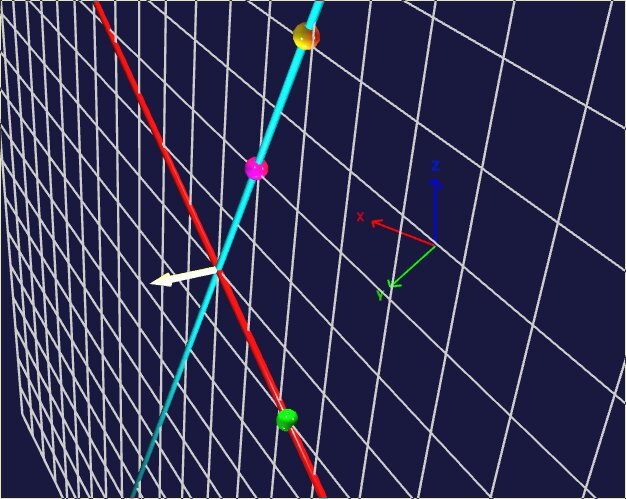
\includegraphics[width = 0.9\textwidth]{\fig/l4_es2.jpeg}
\end{center}
\end{frame}
%

\end{document}
